\begin{exercise}
	Δείξτε ότι ισχύει η αντιμεταθετική ιδιότητα για τα ακόλουθα ζευγάρια μετασχηματισμών.
	\begin{enumerate}
		\item Αν στο χώρο εφαρμόσουμε συμμετρία ως προς το επίπεδο $xy$ και συμμετρία ως προς το επίπεδο $yz$.
		\item Αν στο επίπεδο εφαρμόσουμε μεταφορά κατά διάνυσμα $\vec{v}$ και συμετρία ως προς τον άξονα $y$.
	\end{enumerate}
\end{exercise}


%\begin{solution}
%	
%\begin{figure}[hbt]
%  \begin{center}
%	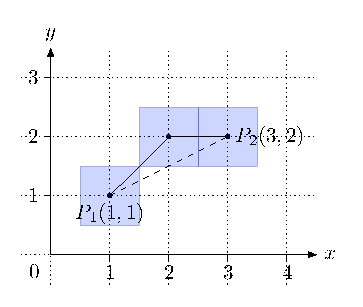
\includegraphics[scale=0.7]{Chapter1/Exercises/ex16/graph1.pdf}
%  \end{center}
%%  \caption{\textcolor{red}{what}}
%\end{figure}	
%	
%\begin{figure}[hbt]
%  \begin{center}
%	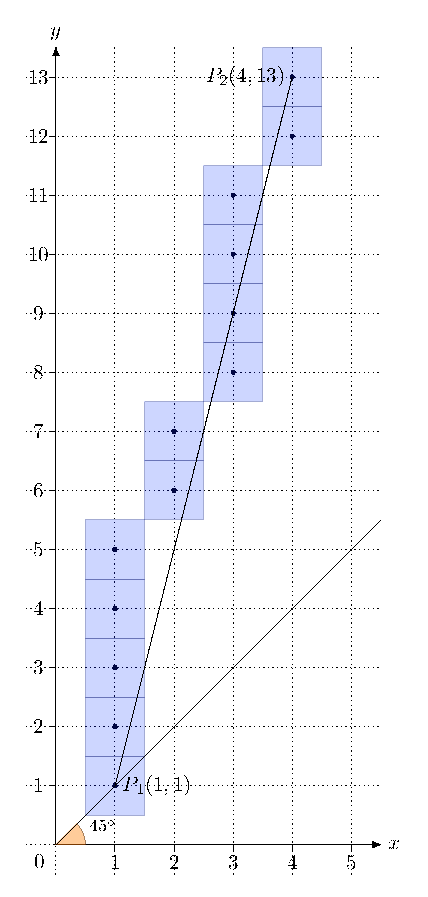
\includegraphics[scale=0.7]{Chapter1/Exercises/ex16/graph2.pdf}
%  \end{center}
%%  \caption{Παράσταση ζητούμενων ευθυγ\textcolor{red}{what}ράμμων τμημάτων}
%\end{figure}	
%	
%\begin{figure}[hbt]
%  \begin{center}
%	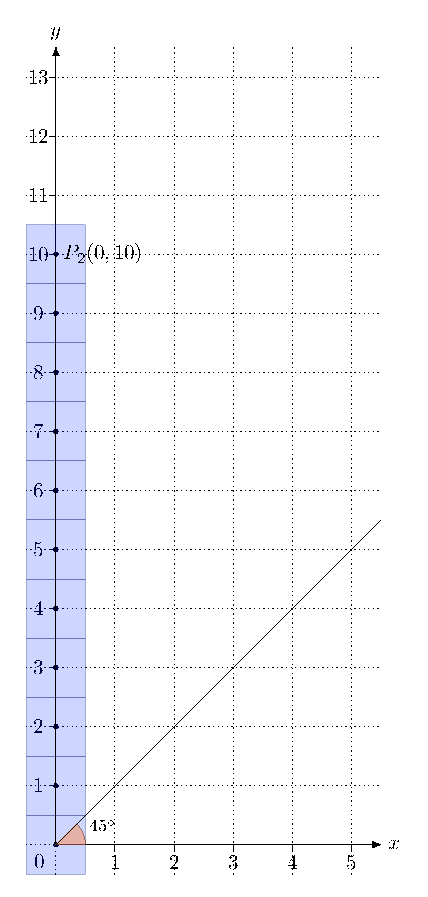
\includegraphics[scale=0.7]{Chapter1/Exercises/ex16/graph3.pdf}
%  \end{center}
%%  \caption{Παράσταση ζητούμενων ευθυγ\textcolor{red}{what}ράμμων τμημάτων}
%\end{figure}		
%	
%	
%\begin{align*}
%    \begin{minipage}{0.4\textwidth}
%        \begin{tikzpicture}
%            \draw[step=1.5cm, line width=0.5mm, gray!10!gray] (0,0) grid (4.5,4.5);
%            \draw[step=1.5cm, line width=0.6mm, black!10!black] (1.5,0) grid (4.5,3);
%            \draw [pattern={Lines[angle=45,distance=4pt,]},pattern color=orange]  (3.75,0.75) circle [radius=0.75];
%            \draw (3.7,0) arc [x radius= 8, y radius= 8.5, start angle=0, end angle=32];
%            \foreach \x in {0.75,2.25,3.75} {
%                \node [fill= gray, fill opacity=0.1, draw=none, thick, minimum size=1.5cm] at (\x,0.75);
%                \node [fill= gray, fill opacity=0.1, draw=none, thick, minimum size=1.5cm] at (\x,2.25);
%                \node [fill= gray, fill opacity=0.1, draw=none, thick, minimum size=1.5cm] at (\x,3.75);
%                }
%            \node[anchor=east] at (0,0.75) {\Large $0$};
%            \node[anchor=east] at (0,2.25) {\Large $1$};
%            \node[anchor=east] at (0,3.75) {\Large $2$};
%            \node[anchor=north] at (0.75,0) {\Large $3$};
%            \node[anchor=north] at (2.25,0) {\Large $4$};
%            \node[anchor=north] at (3.75,0) {\Large $5$};
%            \node at (2.25,2.25) {\large $C$};
%            \node at (3.75,2.25) {\large $D$};
%            \node[anchor=south] at (2.7,3) {\large $M$};
%            \node[anchor=south] at (3.4,3) {\large $T$};
%            \node[anchor=south] at (3.3,4.5) {\large \color{white} $T$};
%            \node[anchor=south] at (2.25,4.5) {\large \color{white} $ t$};
%        \end{tikzpicture}
%    \end{minipage}
%    \begin{minipage}{0.4\textwidth}
%        \begin{tikzpicture}
%            \draw[step=1.5cm, line width=0.5mm, gray!10!gray] (0,0) grid (4.5,4.5);
%            \draw[step=1.5cm, line width=0.6mm, black!10!black] (1.5,1.5) grid (4.5,4.5);
%            \draw [pattern={Lines[angle=45,distance=4pt,]},pattern color=orange]  (3.75,0.75) circle [radius=0.75];
%            \draw [pattern={Lines[angle=45,distance=4pt,]},pattern color=orange]  (3.75,2.25) circle [radius=0.75];
%            \draw (3.7,0) arc [x radius= 8, y radius= 8.5, start angle=0, end angle=32];
%            \foreach \x in {0.75,2.25,3.75} {
%                \node [fill= gray, fill opacity=0.1, draw=none, thick, minimum size=1.5cm] at (\x,0.75);
%                \node [fill= gray, fill opacity=0.1, draw=none, thick, minimum size=1.5cm] at (\x,2.25);
%                \node [fill= gray, fill opacity=0.1, draw=none, thick, minimum size=1.5cm] at (\x,3.75);
%                }
%            \node[anchor=east] at (0,0.75) {\Large $0$};
%            \node[anchor=east] at (0,2.25) {\Large $1$};
%            \node[anchor=east] at (0,3.75) {\Large $2$};
%            \node[anchor=north] at (0.75,0) {\Large $3$};
%            \node[anchor=north] at (2.25,0) {\Large $4$};
%            \node[anchor=north] at (3.75,0) {\Large $5$};
%            \node at (2.25,3.75) {\large $C$};
%            \node at (3.75,3.75) {\large $D$};
%            \node[anchor=south] at (3.3,4.5) {\large $M$};
%            \node[anchor=south] at (2.25,4.5) {\large $T$};
%        \end{tikzpicture}
%    \end{minipage}
%    \begin{minipage}{0.4\textwidth}
%        \begin{tikzpicture}
%            \draw[step=1.5cm, line width=0.5mm, gray!10!gray] (0,0) grid (4.5,4.5);
%            \draw [pattern={Lines[angle=45,distance=4pt,]},pattern color=orange]  (3.75,0.75) circle [radius=0.75];
%            \draw [pattern={Lines[angle=45,distance=4pt,]},pattern color=orange]  (3.75,2.25) circle [radius=0.75];
%            \draw [pattern={Lines[angle=45,distance=4pt,]},pattern color=orange]  (2.25,3.75) circle [radius=0.75];
%            \draw (3.7,0) arc [x radius= 8, y radius= 8.5, start angle=0, end angle=32];
%            \foreach \x in {0.75,2.25,3.75} {
%                \node [fill= gray, fill opacity=0.1, draw=none, thick, minimum size=1.5cm] at (\x,0.75);
%                \node [fill= gray, fill opacity=0.1, draw=none, thick, minimum size=1.5cm] at (\x,2.25);
%                \node [fill= gray, fill opacity=0.1, draw=none, thick, minimum size=1.5cm] at (\x,3.75);
%                }
%            \node[anchor=east] at (0,0.75) {\Large $0$};
%            \node[anchor=east] at (0,2.25) {\Large $1$};
%            \node[anchor=east] at (0,3.75) {\Large $2$};
%            \node[anchor=north] at (0.75,0) {\Large $3$};
%            \node[anchor=north] at (2.25,0) {\Large $4$};
%            \node[anchor=north] at (3.75,0) {\Large $5$};
%            \node[anchor=south] at (3.3,4.5) {\large \color{white} $T$};
%            \node[anchor=south] at (2.25,4.5) {\large \color{white} $ t$};
%        \end{tikzpicture}
%    \end{minipage}
%\end{align*}
%\begin{align*}
%    f_{mid1,1} = a^2 - b^2 a + \frac{b^2}{4} \overset{a=5,b=3}{=} 25 - 45 + \frac{9}{4}= -17.75 < 0 
%\end{align*} 
%Άρα φωτίζεται το $pixel$ στην θέση $(5,1)$. Έχουμε δείξει ότι ο αναδρομικός τύπος του $f_{mid1,i}$ είναι:
%\begin{center}
%    \begin{tabular}{ |c|c|c| } 
%        \hline
%        $f_{mid1,i}<0$ &$ f_{mid1,i} +2a^2 (y_{i}+1) + a^2$& Επιλογή σημείου $D$\\
%        \hline
%        $f_{mid1,i} \geq 0$ &$ f_{mid1,i} +2a^2 (y_{i}+1) + a^2 -2b^2(x_{i}-1)$& Επιλογή σημείου $C$\\
%        \hline  
%    \end{tabular}
%\end{center}
%Άρα έχουμε ότι:
%\begin{align*}
%     f_{mid1,2} = f_{mid1,1} + 2a^2 (y_{i}+1) + a^2 \overset{a=5}{=} -17.75 + 75 = 57.25 > 0 
%\end{align*}
%Άρα φωτίζεται το $pixel$ στην θέση $(4,2)$. Ελέγχουμε αν έχουμε περάσει στην περιοχή 2:
%\begin{align*}
%     2b^2x > 2a^2y \overset{a=5,b=3}{\Rightarrow} 72\ngtr100 
%\end{align*}
%άρα περάσαμε στην περιοχή 2. Υπολογίζουμε το $f_{mid2,1}$:
%\begin{align*}
%    f_{mid2,1} = f_ {mid1,2} - \frac {(2b^ {2}x_ {3}+2a^ {2}y_ {3})}{2}  +0.75(  b^ {2}  -  a^ {2} ) = 57.25 - 86 -12 = -40.75 < 0 
%\end{align*}
%Άρα φωτίζεται το $pixel$ στην θέση $(3,3)$. Έχουμε δείξει ότι ο αναδρομικός τύπος του $f_{mid2,i}$ είναι:
%\begin{center}
%    \begin{tabular}{ |c|c| } 
%        \hline
%        $f_{mid2,i}<0$ &$ f_{mid2,i} -2b^2 (x_{i}-1) + b^2 + 2a^2 (y_{i}+1)$\\
%        \hline
%        $f_{mid2,i} \geq 0$ &$ f_{mid2,i} -2b^2 (x_{i}-1) + b^2 $\\
%        \hline  
%    \end{tabular}
%\end{center}
%Άρα έχουμε ότι:
%\begin{align*}
%   f_{mid2,2} = f_{mid2,1} -2b^2 (x_{3}-1) + b^2 = -40.75 - 32 +9 + 150 = 86.25 > 0 
%\end{align*}
%Άρα φωτίζεται το $pixel$ στην θέση $(3,2)$.
%
%\begin{figure}[hbt]
%  \begin{center}
%	\includegraphics[scale=0.7]{Chapter1/Exercises/ex16/graph4.pdf}
%  \end{center}
%%  \caption{\textcolor{red}{what}}
%\end{figure}	
%	
%\begin{figure}[hbt]
%  \begin{center}
%	\includegraphics[scale=0.7]{Chapter1/Exercises/ex16/graph5.pdf}
%  \end{center}
%%  \caption{Παράσταση ζητούμενων ευθυγ\textcolor{red}{what}ράμμων τμημάτων}
%\end{figure}	
%	
%\begin{figure}[hbt]
%  \begin{center}
%	\includegraphics[scale=0.7]{Chapter1/Exercises/ex16/graph6.pdf}
%  \end{center}
%%  \caption{Παράσταση ζητούμενων ευθυγ\textcolor{red}{what}ράμμων τμημάτων}
%\end{figure}
%
%\begin{figure}[hbt]
%  \begin{center}
%	\includegraphics[scale=0.7]{Chapter1/Exercises/ex16/graph7.pdf}
%  \end{center}
%%  \caption{Παράσταση ζητούμενων ευθυγ\textcolor{red}{what}ράμμων τμημάτων}
%\end{figure}
%
%\begin{align*}
%    \begin{minipage}{0.4\textwidth}
%        \begin{tikzpicture}
%            \draw[step=1.5cm, line width=0.5mm, gray!10!gray] (0,0) grid (4.5,4.5);
%            \draw[step=1.5cm, line width=0.6mm, black!10!black] (1.5,0) grid (4.5,3);
%            \draw [pattern={Lines[angle=45,distance=4pt,]},pattern color=orange]  (3.75,0.75) circle [radius=0.75];
%            \draw (3.7,0) arc [x radius= 4.2, y radius= 4.5, start angle=28, end angle=90];
%            \foreach \x in {0.75,2.25,3.75} {
%                \node [fill= gray, fill opacity=0.1, draw=none, thick, minimum size=1.5cm] at (\x,0.75);
%                \node [fill= gray, fill opacity=0.1, draw=none, thick, minimum size=1.5cm] at (\x,2.25);
%                \node [fill= gray, fill opacity=0.1, draw=none, thick, minimum size=1.5cm] at (\x,3.75);
%                }
%            \node[anchor=east] at (0,0.75) {\Large $2$};
%            \node[anchor=east] at (0,2.25) {\Large $3$};
%            \node[anchor=east] at (0,3.75) {\Large $4$};
%            \node[anchor=north] at (0.75,0) {\Large $2$};
%            \node[anchor=north] at (2.25,0) {\Large $3$};
%            \node[anchor=north] at (3.75,0) {\Large $4$};
%            \node at (2.25,2.25) {\large $C$};
%            \node at (2.25,0.75) {\large $B$};
%            \node[anchor=east] at (1.5,1.75) {\large $M$};
%            \node[anchor=east] at (1.5,2.5) {\large $T$};
%            \node[anchor=south] at (3.3,4.5) {\large \color{white} $T$};
%            \node[anchor=south] at (2.25,4.5) {\large \color{white} $ t$};
%        \end{tikzpicture}
%    \end{minipage}
%    \begin{minipage}{0.4\textwidth}
%        \begin{tikzpicture}
%            \draw[step=1.5cm, line width=0.5mm, gray!10!gray] (0,0) grid (4.5,4.5);
%            \draw[step=1.5cm, line width=0.6mm, black!10!black] (0,1.5) grid (3,4.5);
%            \draw [pattern={Lines[angle=45,distance=4pt,]},pattern color=orange]  (3.75,0.75) circle [radius=0.75];
%            \draw [pattern={Lines[angle=45,distance=4pt,]},pattern color=orange]  (2.25,2.25) circle [radius=0.75];
%            \draw (3.7,0) arc [x radius= 4.2, y radius= 4.5, start angle=28, end angle=90];
%            \foreach \x in {0.75,2.25,3.75} {
%                \node [fill= gray, fill opacity=0.1, draw=none, thick, minimum size=1.5cm] at (\x,0.75);
%                \node [fill= gray, fill opacity=0.1, draw=none, thick, minimum size=1.5cm] at (\x,2.25);
%                \node [fill= gray, fill opacity=0.1, draw=none, thick, minimum size=1.5cm] at (\x,3.75);
%                }
%            \node[anchor=east] at (0,0.75) {\Large $2$};
%            \node[anchor=east] at (0,2.25) {\Large $3$};
%            \node[anchor=east] at (0,3.75) {\Large $4$};
%            \node[anchor=north] at (0.75,0) {\Large $2$};
%            \node[anchor=north] at (2.25,0) {\Large $3$};
%            \node[anchor=north] at (3.75,0) {\Large $4$};
%            \node at (0.75,3.75) {\large $C$};
%            \node at (0.75,2.25) {\large $B$};
%            \node[anchor=east] at (0,3) {\large $M$};
%            \node[anchor=west] at (0,2.6) {\large $T$};
%            \node[anchor=south] at (3.3,4.5) {\large \color{white} $T$};
%            \node[anchor=south] at (2.25,4.5) {\large \color{white} $ t$};
%        \end{tikzpicture}
%    \end{minipage}
%    \begin{minipage}{0.4\textwidth}
%        \begin{tikzpicture}
%            \draw[step=1.5cm, line width=0.5mm, gray!10!gray] (0,0) grid (4.5,4.5);
%            \draw [pattern={Lines[angle=45,distance=4pt,]},pattern color=orange]  (3.75,0.75) circle [radius=0.75];
%            \draw [pattern={Lines[angle=45,distance=4pt,]},pattern color=orange]  (2.25,2.25) circle [radius=0.75];
%            \draw [pattern={Lines[angle=45,distance=4pt,]},pattern color=orange]  (0.75,2.25) circle [radius=0.75];
%            \draw (3.7,0) arc [x radius= 4.2, y radius= 4.5, start angle=28, end angle=90];
%            \foreach \x in {0.75,2.25,3.75} {
%                \node [fill= gray, fill opacity=0.1, draw=none, thick, minimum size=1.5cm] at (\x,0.75);
%                \node [fill= gray, fill opacity=0.1, draw=none, thick, minimum size=1.5cm] at (\x,2.25);
%                \node [fill= gray, fill opacity=0.1, draw=none, thick, minimum size=1.5cm] at (\x,3.75);
%                }
%            \node[anchor=east] at (0,0.75) {\Large $2$};
%            \node[anchor=east] at (0,2.25) {\Large $3$};
%            \node[anchor=east] at (0,3.75) {\Large $4$};
%            \node[anchor=north] at (0.75,0) {\Large $2$};
%            \node[anchor=north] at (2.25,0) {\Large $3$};
%            \node[anchor=north] at (3.75,0) {\Large $4$};
%            \node[anchor=south] at (3.3,4.5) {\large \color{white} $T$};
%            \node[anchor=south] at (2.25,4.5) {\large \color{white} $ t$};
%        \end{tikzpicture}
%    \end{minipage}
%\end{align*}
%Το συνολικό σχήμα που φωτίστηκε είναι το παρακάτω.
%\begin{align*}
%    \begin{tikzpicture}[x=1cm, y=1cm]
%        \draw[step=1.5cm, line width=0.5mm, gray!10!gray] (0,0) grid (6,6);      
%        \draw [pattern={Lines[angle=45,distance=4pt,]},pattern color=orange]  (5.25,0.75) circle [radius=0.75];
%        \draw [pattern={Lines[angle=45,distance=4pt,]},pattern color=orange]  (5.25,2.25) circle [radius=0.75];
%        \draw [pattern={Lines[angle=45,distance=4pt,]},pattern color=orange]  (3.75,3.75) circle [radius=0.75];
%        \draw [pattern={Lines[angle=45,distance=4pt,]},pattern color=orange]  (2.25,5.25) circle [radius=0.75];
%        \draw [pattern={Lines[angle=45,distance=4pt,]},pattern color=orange]  (0.75,5.25) circle [radius=0.75];
%        \node[anchor=east] at (0,0.75) {\Large $0$};
%        \node[anchor=east] at (0,2.25) {\Large $1$};
%        \node[anchor=east] at (0,3.75) {\Large $2$};
%        \node[anchor=east] at (0,5.25) {\Large $3$};
%        \node[anchor=north] at (0.75,0) {\Large $2$};
%        \node[anchor=north] at (2.25,0) {\Large $3$};
%        \node[anchor=north] at (3.75,0) {\Large $4$};
%        \node[anchor=north] at (5.25,0) {\Large $5$};
%        \node at (3.75,1.5) {\Huge \color{blue}$1$};
%        \node at (1.5,3.75) {\Huge \color{blue}$2$};
%        \draw[scale=0.5, domain=0:12, smooth, variable=\x, blue] plot ({\x}, {\x});
%        \foreach \x in {0.75,2.25,3.75,5.25} {
%                \node [fill= gray, fill opacity=0.1, draw=none, thick, minimum size=1.5cm] at (\x,0.75);
%                \node [fill= gray, fill opacity=0.1, draw=none, thick, minimum size=1.5cm] at (\x,2.25);
%                \node [fill= gray, fill opacity=0.1, draw=none, thick, minimum size=1.5cm] at (\x,3.75);
%                \node [fill= gray, fill opacity=0.1, draw=none, thick, minimum size=1.5cm] at (\x,5.25);
%                }
%    \end{tikzpicture}
%\end{align*}
%
%\end{solution}